\begin{flushleft}
Seleccionamos la opción Clase de Escritorio y luego en el botón siguiente\\
\begin{center}
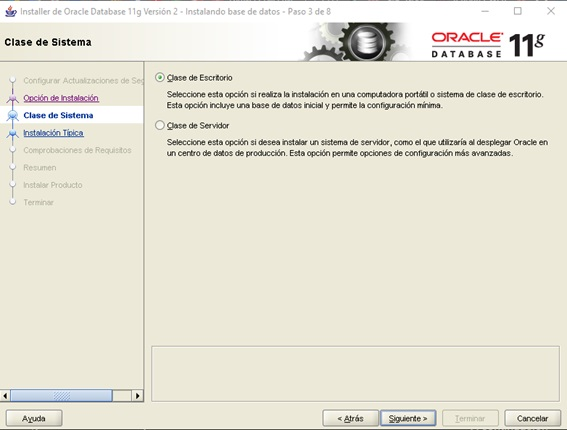
\includegraphics{images/image-08}\\
\end{center}
En esta parte de la instalación llenamos todo el formulario y luego en el botón siguiente\\
\begin{center}
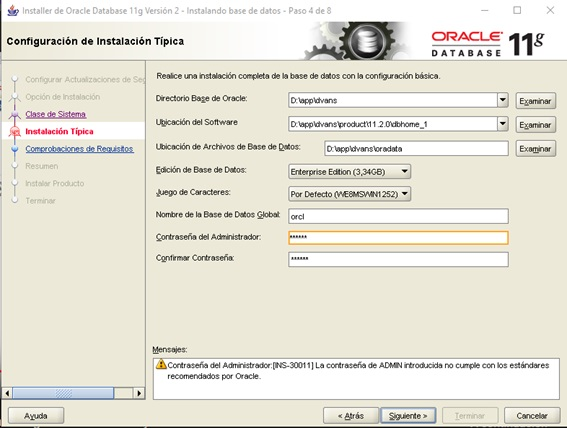
\includegraphics{images/image-09}\\
\end{center}
En caso de introducir una clave que no cumpla con los estándares nos saldrá esta ventana y colocamos en que si, para confirmar que estamos seguros de continuar.\\
\begin{center}
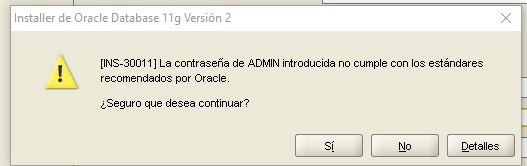
\includegraphics{images/image-10}\\
\end{center}
En esta ventana presionamos en el botón terminar\\
\begin{center}
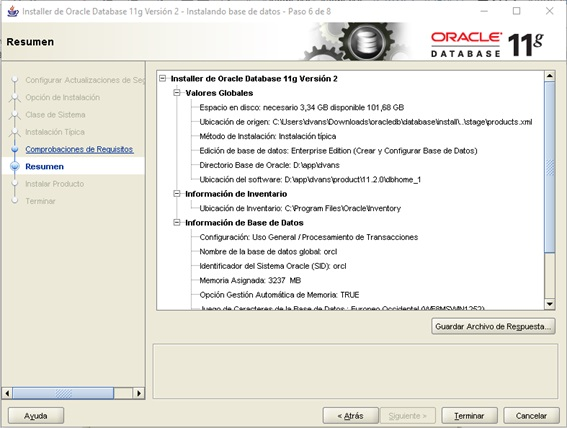
\includegraphics{images/image-11}\\
\end{center}
Luego empezara realizar la instalación\\
\begin{center}
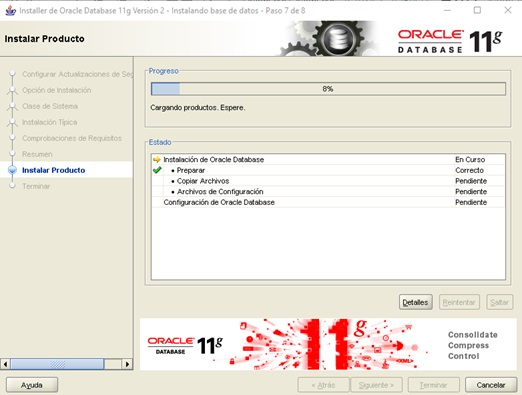
\includegraphics{images/image-12}\\
\end{center}
Adicionalmente aparecerá el asistente de configuración de bases de datos en el cual no debemos parar el proceso de configuración\\
\begin{center}
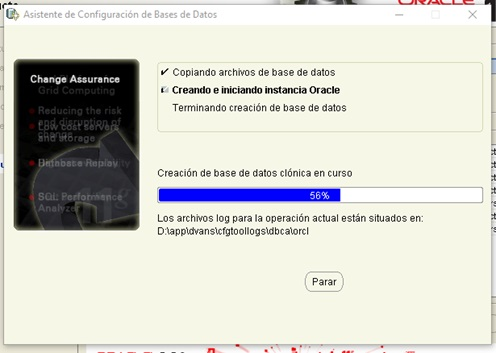
\includegraphics{images/image-13}\\
\end{center}
Una vez terminado la instalación el asistente nos mostrara esta ventana en la que debemos aceptar\\
\begin{center}
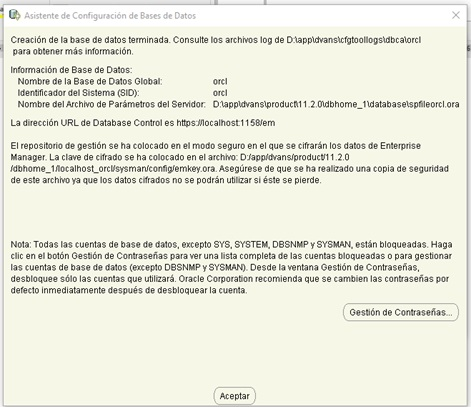
\includegraphics{images/image-14}\\
\end{center}
Finalmente se mostrará esta ventana indicándonos la URL donde se esta ejecutando el ENTERPRISE MANAGE DATABASE CONTROL y para finalizar presionamos el botón cerrar\\
\begin{center}
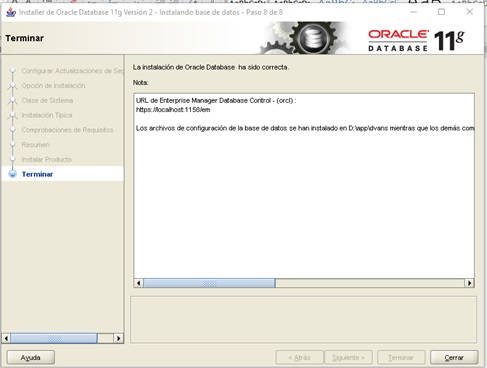
\includegraphics{images/image-15}\\
\end{center}
Abrimos la URL de ENTERPRISE MANAGE DATABASE CONTROL, de modo que comprobamos que la instalación se realizó correctamente. En esta ventana nos pedirá usuario y contraseña, por defecto colocamos “sys” como usuario y “oracle” como como contraseña, luego conectamos presionando en el botón conectar\\
\begin{center}
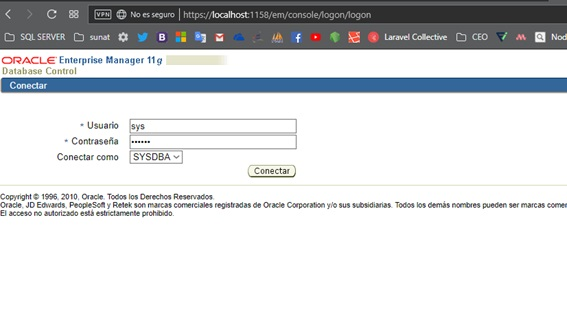
\includegraphics{images/image-16}\\
\end{center}
Una vez logueados correctamente nos aparecerá esta página\\
\begin{center}
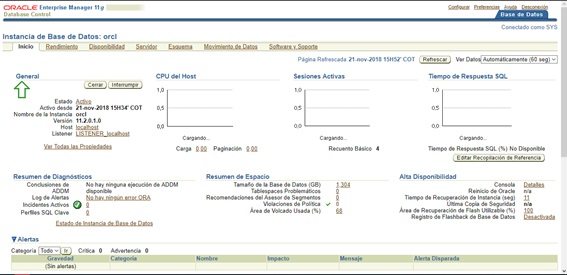
\includegraphics{images/image-17}\\
\end{center}
\end{flushleft}